\section{Discussion}


\subsection{Profile plots}


Figure \ref{fig:Profiles} shows the latitude profiles of the different models in differential flux. The flux increases towards the Galactic plane. Left-right assymmetry close to the Galactic center. 


\begin{figure*}[h!]
    \begin{subfigure}{0.5\textwidth}
        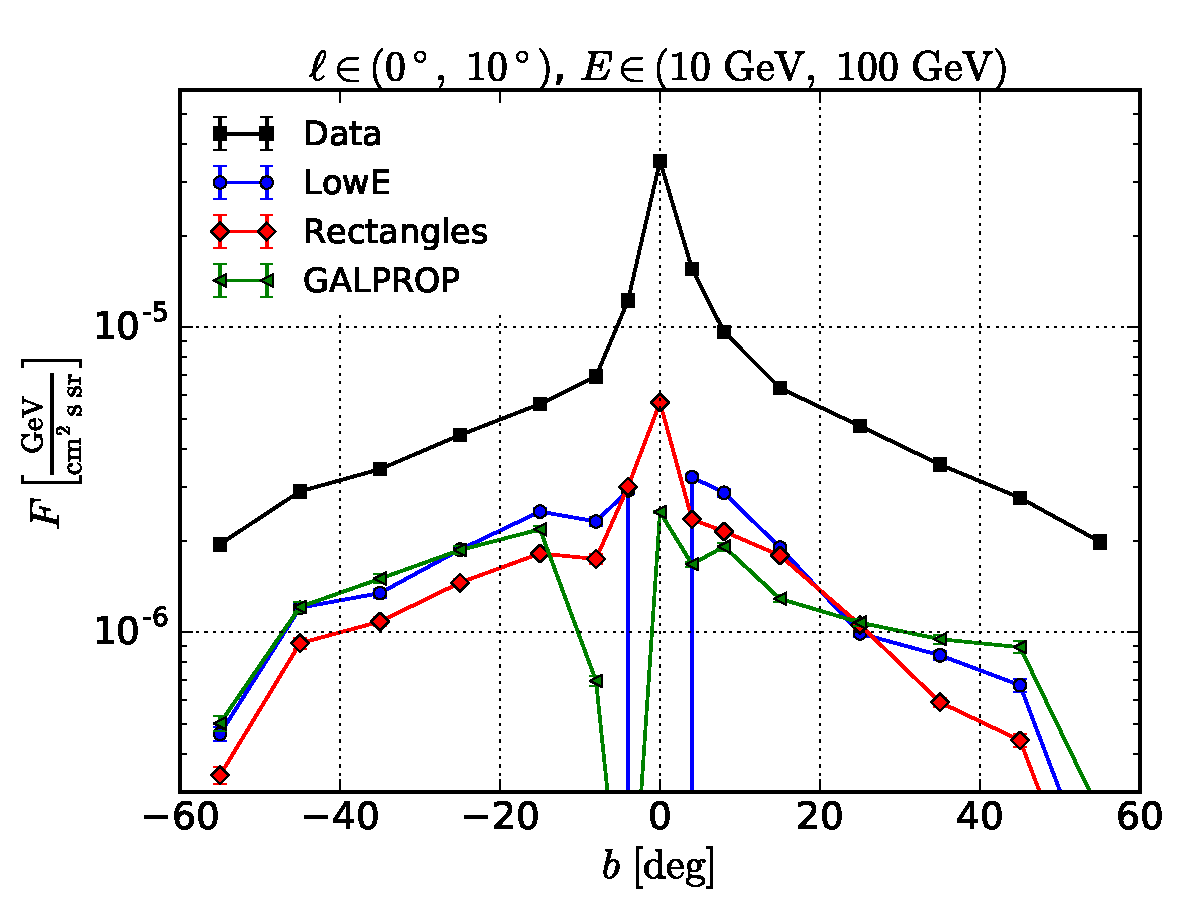
\includegraphics[width=\textwidth]{plots/Profiles_l=1_source_range_1.pdf}
    \end{subfigure} 
    \begin{subfigure}{0.5\textwidth}
        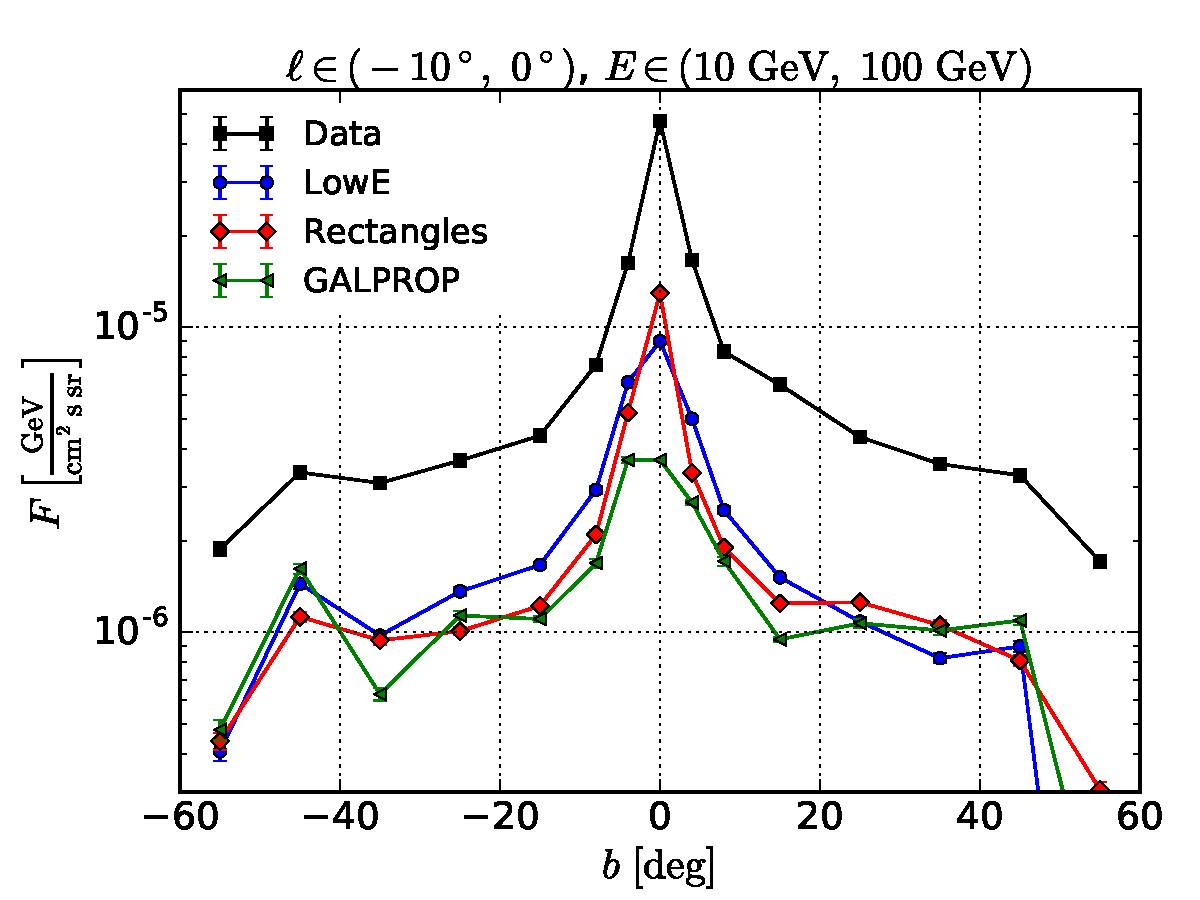
\includegraphics[width=\textwidth]{plots/Profiles_l=0_source_range_1.pdf}
    \end{subfigure}
  	\caption{Latitude profiles of the different models.}
  	\label{fig:Profiles}
\end{figure*}

\subsection{Comparison of the spectra at different latitudes}

Figure \ref{fig:SED_all} shows a comparison of the SED of the raw data (without point sources), the three different models and the difference in the raw data in a very thin latitude stripe covering the Galactic plane. The models give similar results. 


\begin{figure*}[h!]
    \begin{subfigure}{0.5\textwidth}
        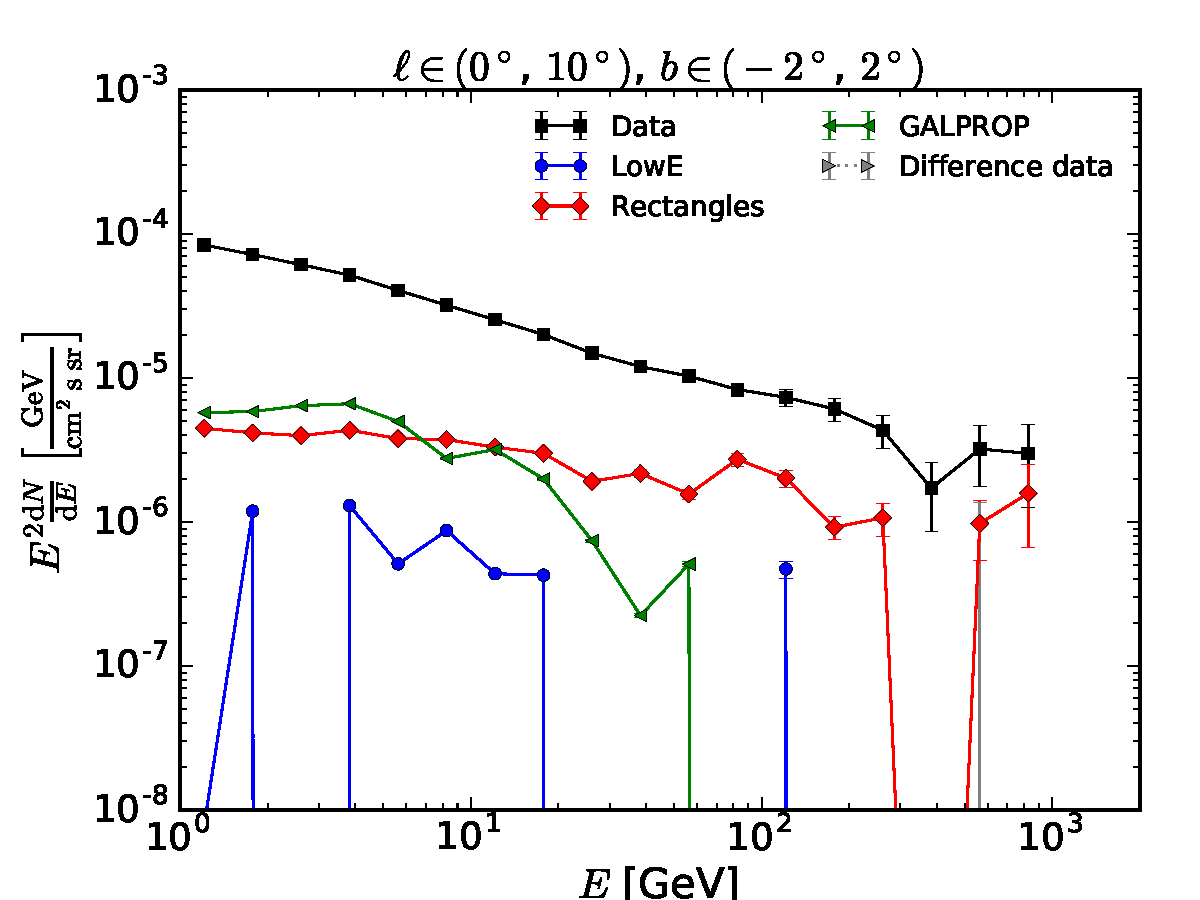
\includegraphics[width=\textwidth]{plots/SED_all_models_source_l=5_b=0.pdf}
    \end{subfigure} 
    \begin{subfigure}{0.5\textwidth}
        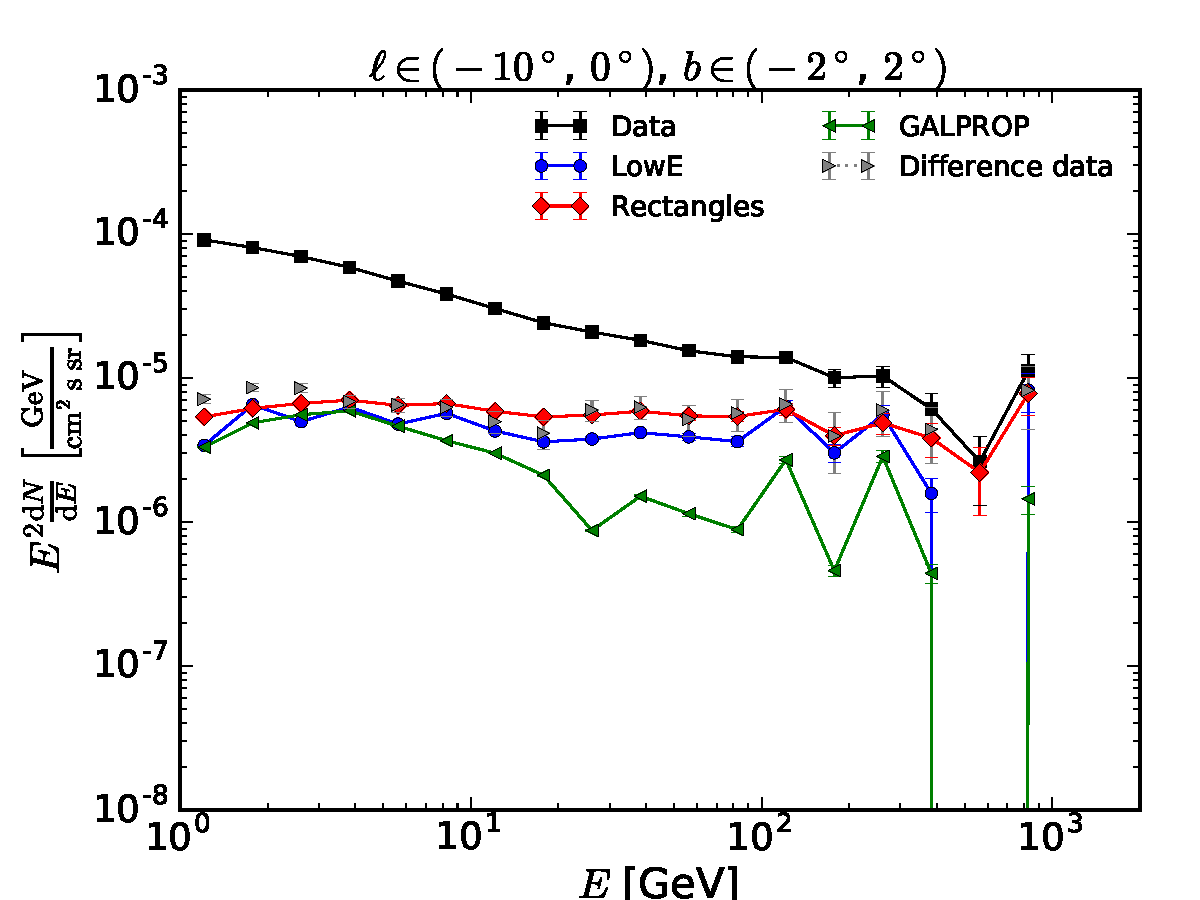
\includegraphics[width=\textwidth]{plots/SED_all_models_source_l=-5_b=0.pdf}
    \end{subfigure}
  	\caption{Comparison of SED of all models.}
  	\label{fig:SED_all}
\end{figure*}

Fit the spectra with a power-law and a cutoff function.
Fit the spectra with IC and pi0 models.

\begin{figure*}[h!]
    \begin{subfigure}{0.5\textwidth}
        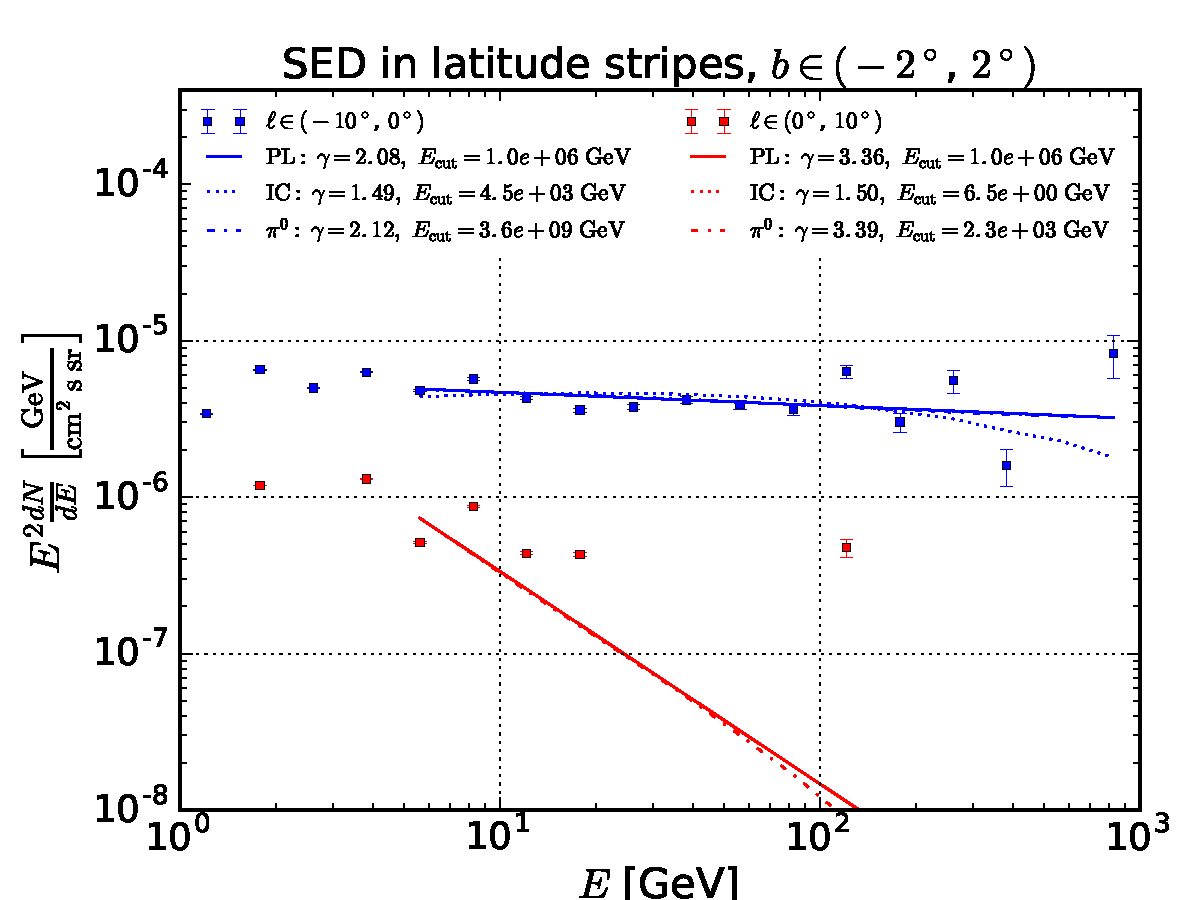
\includegraphics[width=\textwidth]{plots/SED_lowE_source_0cutoff.pdf}
    \end{subfigure} 
    \begin{subfigure}{0.5\textwidth}
        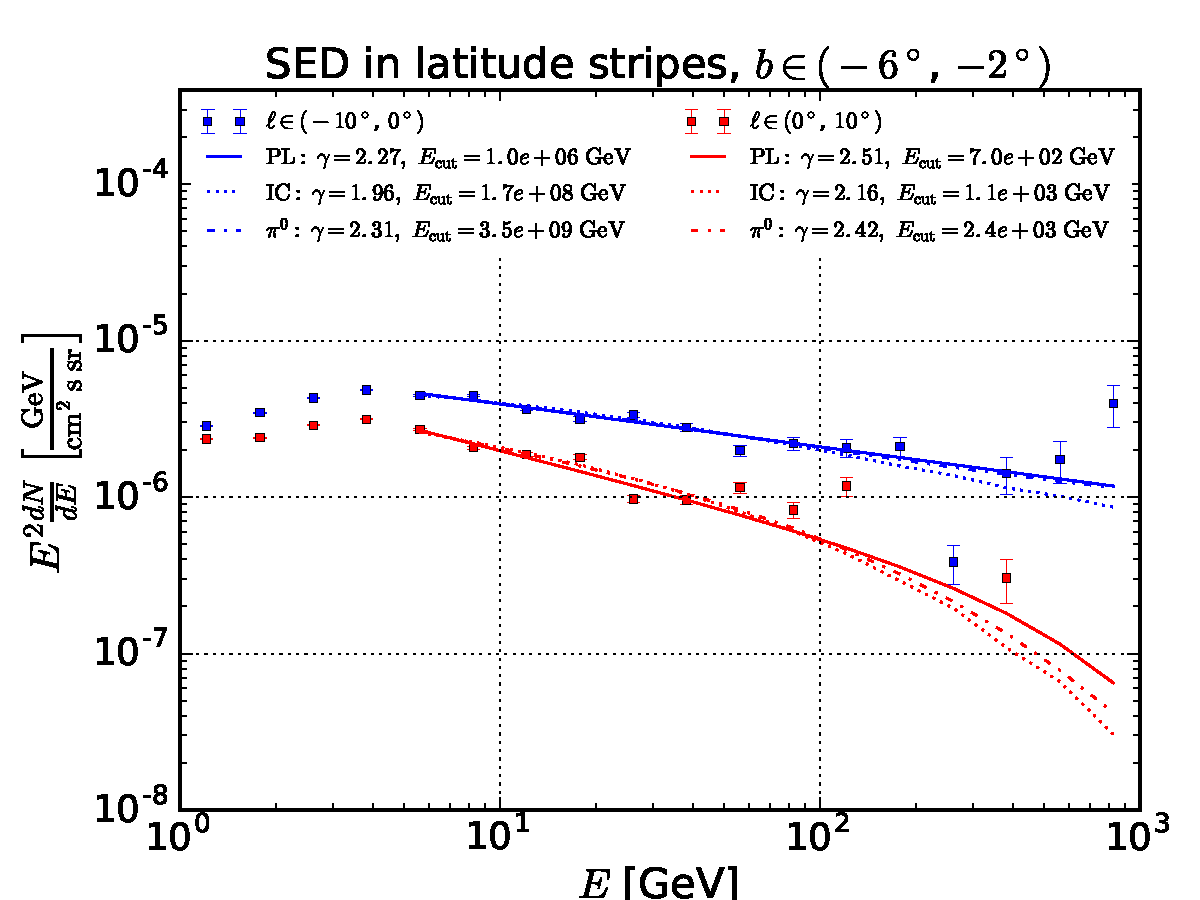
\includegraphics[width=\textwidth]{plots/SED_lowE_source_-4cutoff.pdf}
    \end{subfigure}
  	\caption{SED of low-energy model with powerlaw and particle spectra fits.}
  	\label{fig:SED_all}
\end{figure*}


%\begin{figure*}
%\vspace*{-0.2cm}
%	\makebox[\linewidth][c]{%
%	\vspace*{-0.2cm}
%		\begin{subfigure}[b]{.4\textwidth}
%		\centering 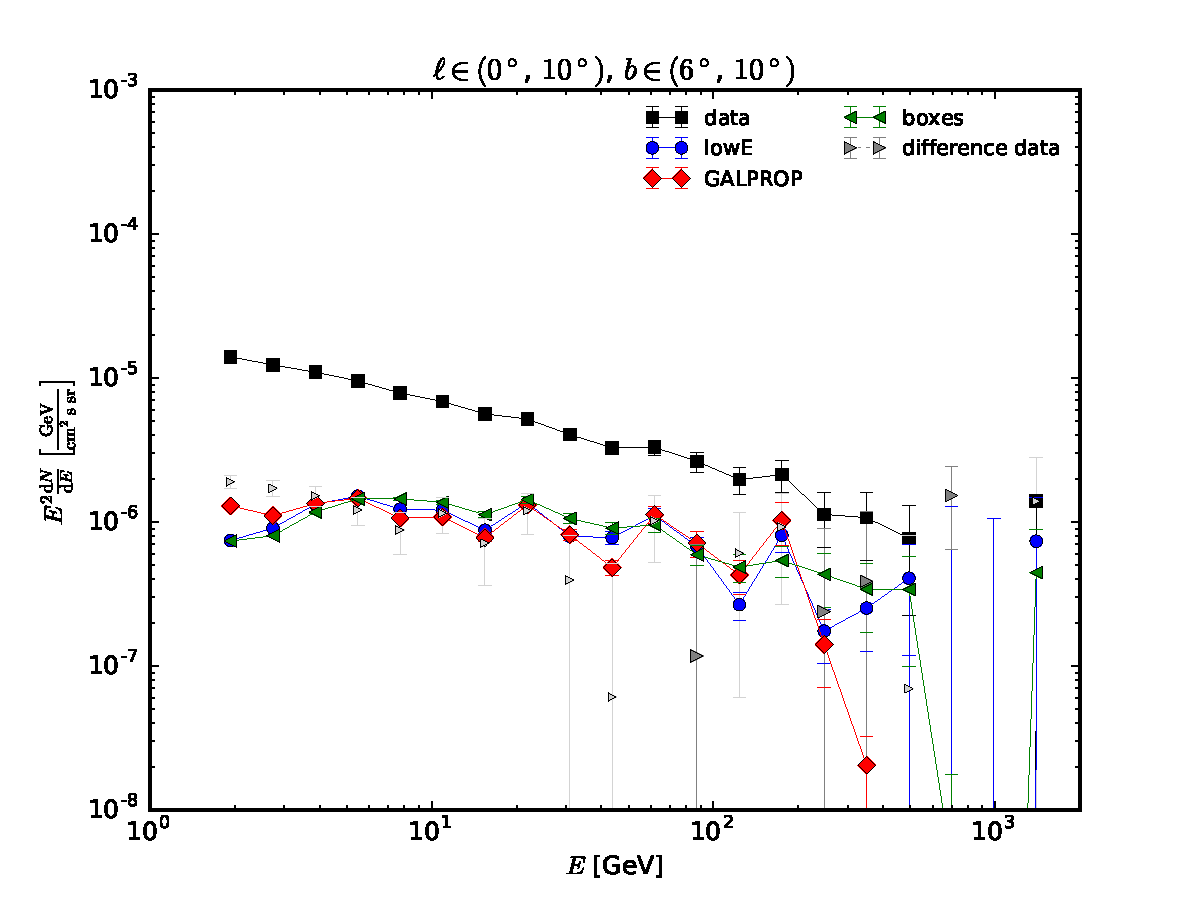
\includegraphics[width=.95\textwidth]{plots/SED_all_left-right__l=5_b=8.pdf}
%		\vspace*{-0.2cm}
%		\end{subfigure}%
%		\begin{subfigure}[b]{.4\textwidth}
%		\centering 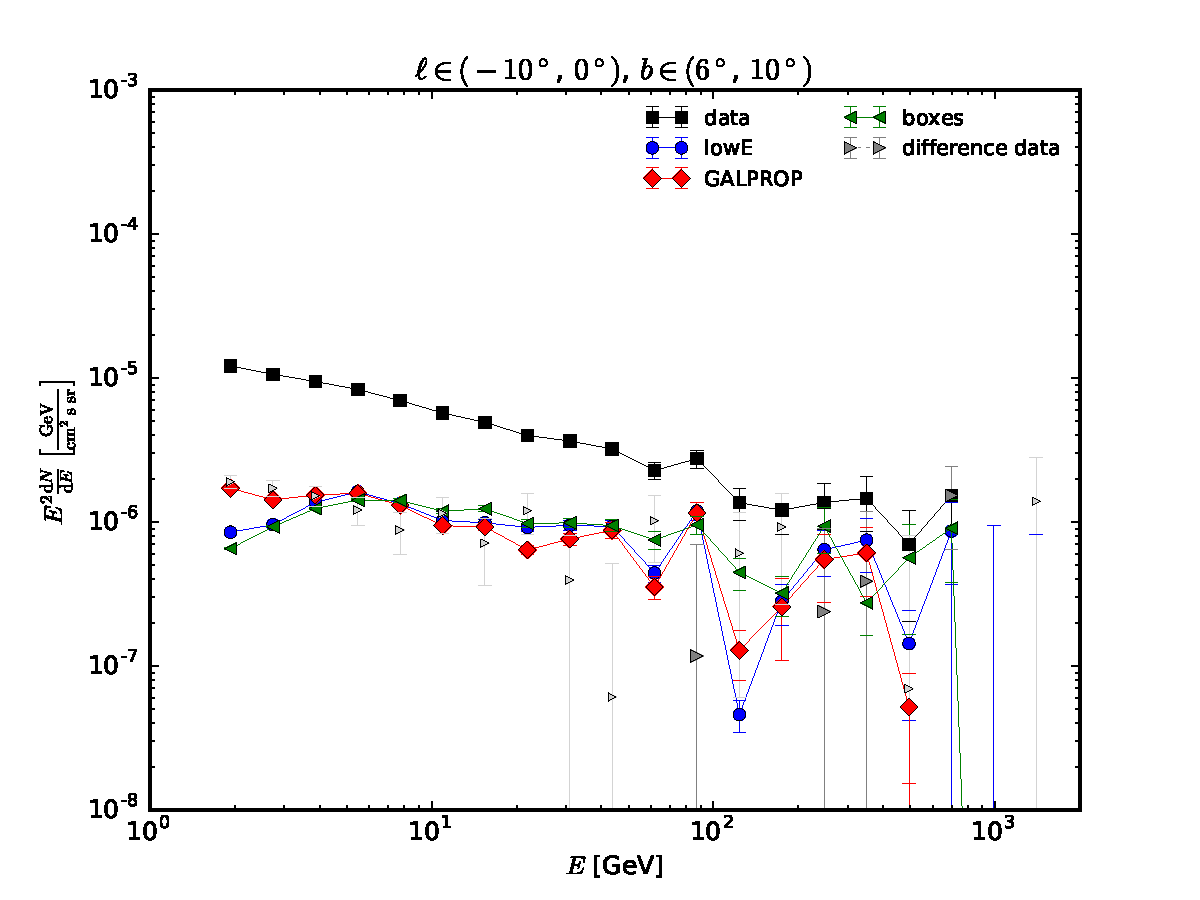
\includegraphics[width=.95\textwidth]{plots/SED_all_left-right__l=-5_b=8.pdf}
%		\vspace*{-0.2cm}
%	\end{subfigure}%
%	\vspace*{-0.2cm}
%	}\\
%	\vspace*{-0.2cm}
%	\makebox[\linewidth][c]{%
%		\begin{subfigure}[b]{.4\textwidth}
%		\centering 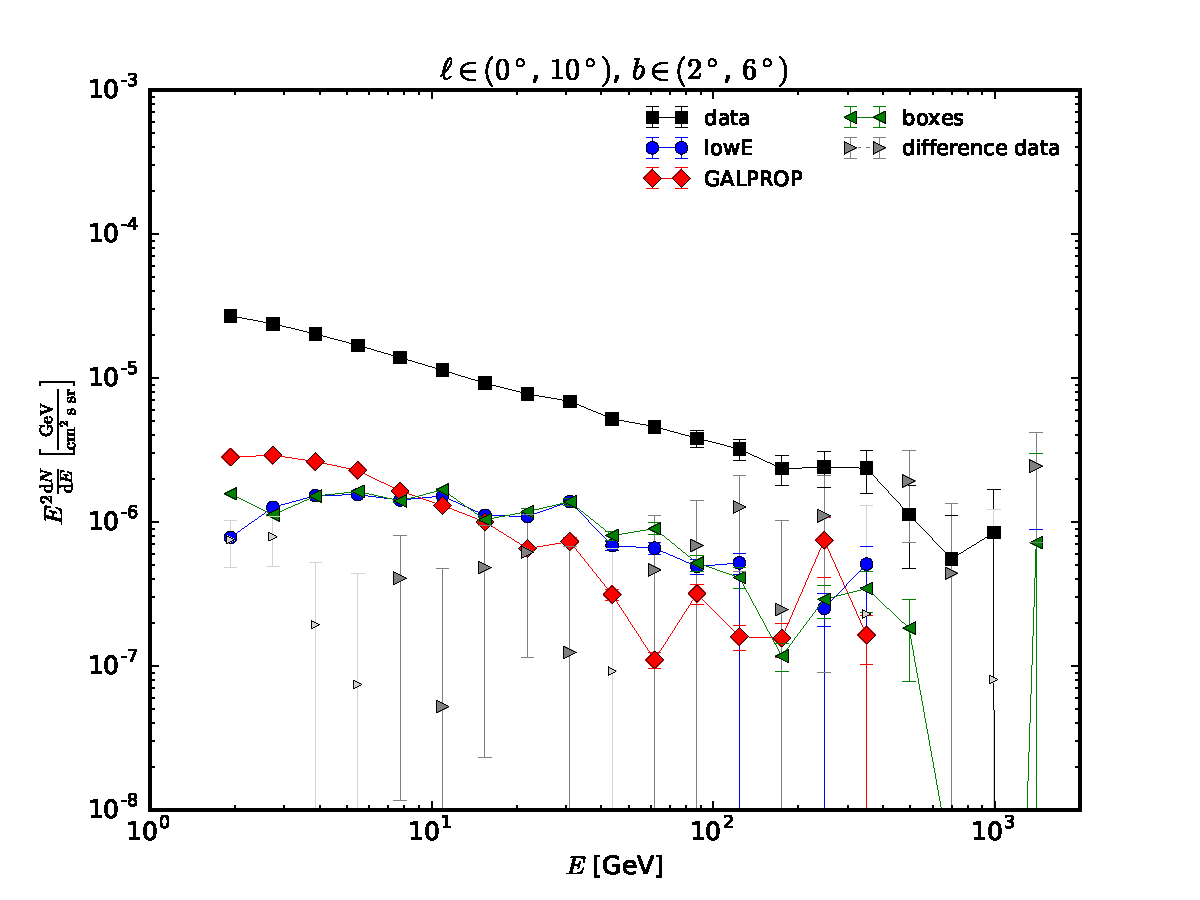
\includegraphics[width=.95\textwidth]{plots/SED_all_left-right__l=5_b=4.pdf}
%		\end{subfigure}%
%		\begin{subfigure}[b]{.4\textwidth}
%		\centering 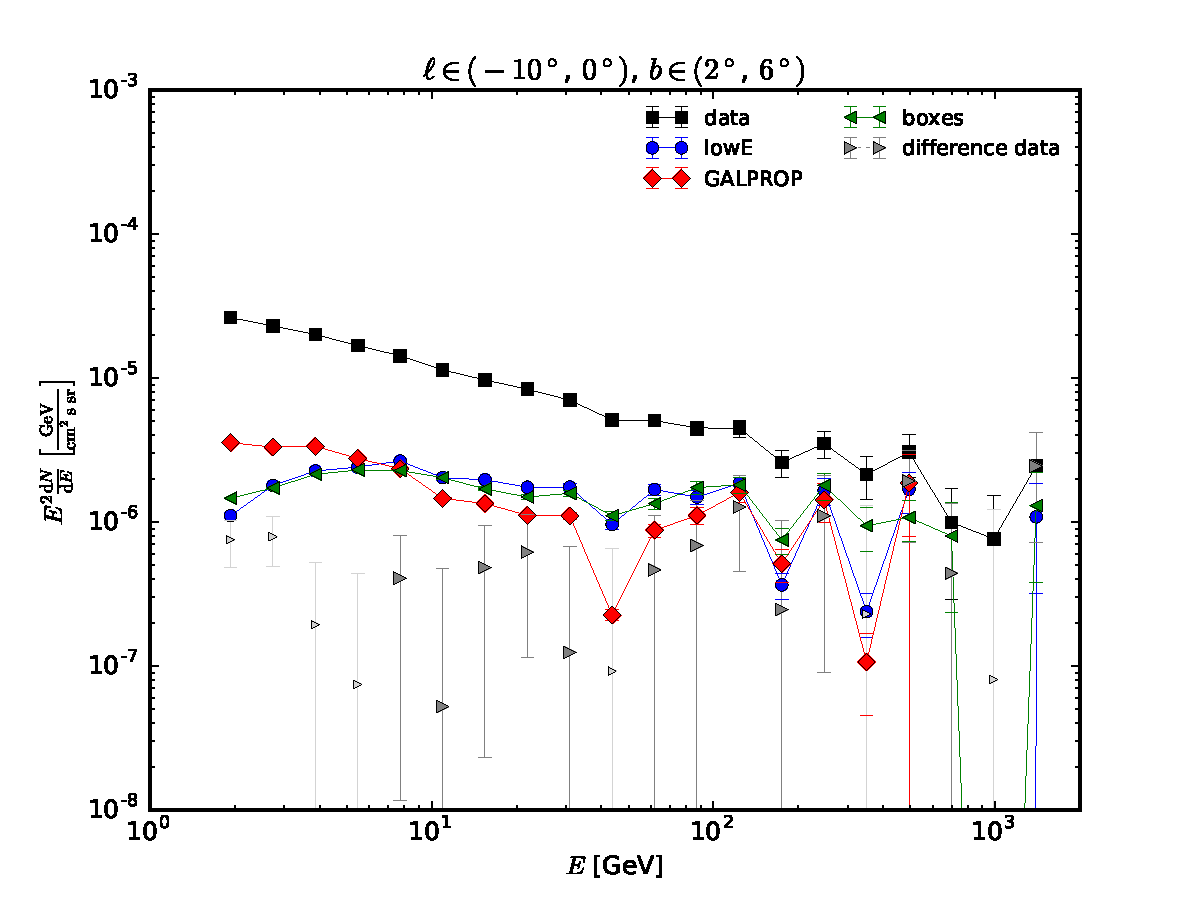
\includegraphics[width=.95\textwidth]{plots/SED_all_left-right__l=-5_b=4.pdf}
%	\end{subfigure}%
%}
%\vspace*{-0.2cm}
%	\makebox[\linewidth][c]{%
%		\begin{subfigure}[b]{.4\textwidth}
%		\centering 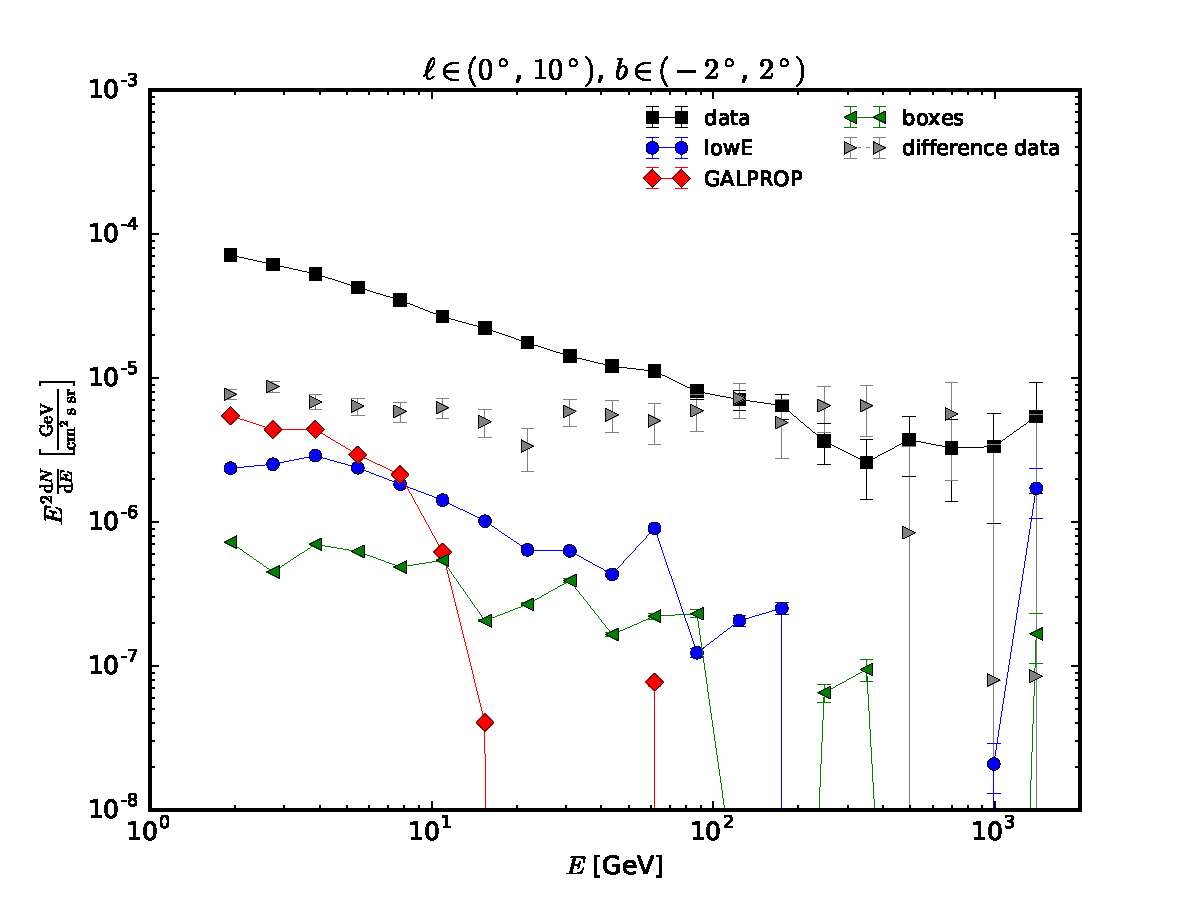
\includegraphics[width=.95\textwidth]{plots/SED_all_left-right__l=5_b=0.pdf}
%		\end{subfigure}%
%		\begin{subfigure}[b]{.4\textwidth}
%		\centering 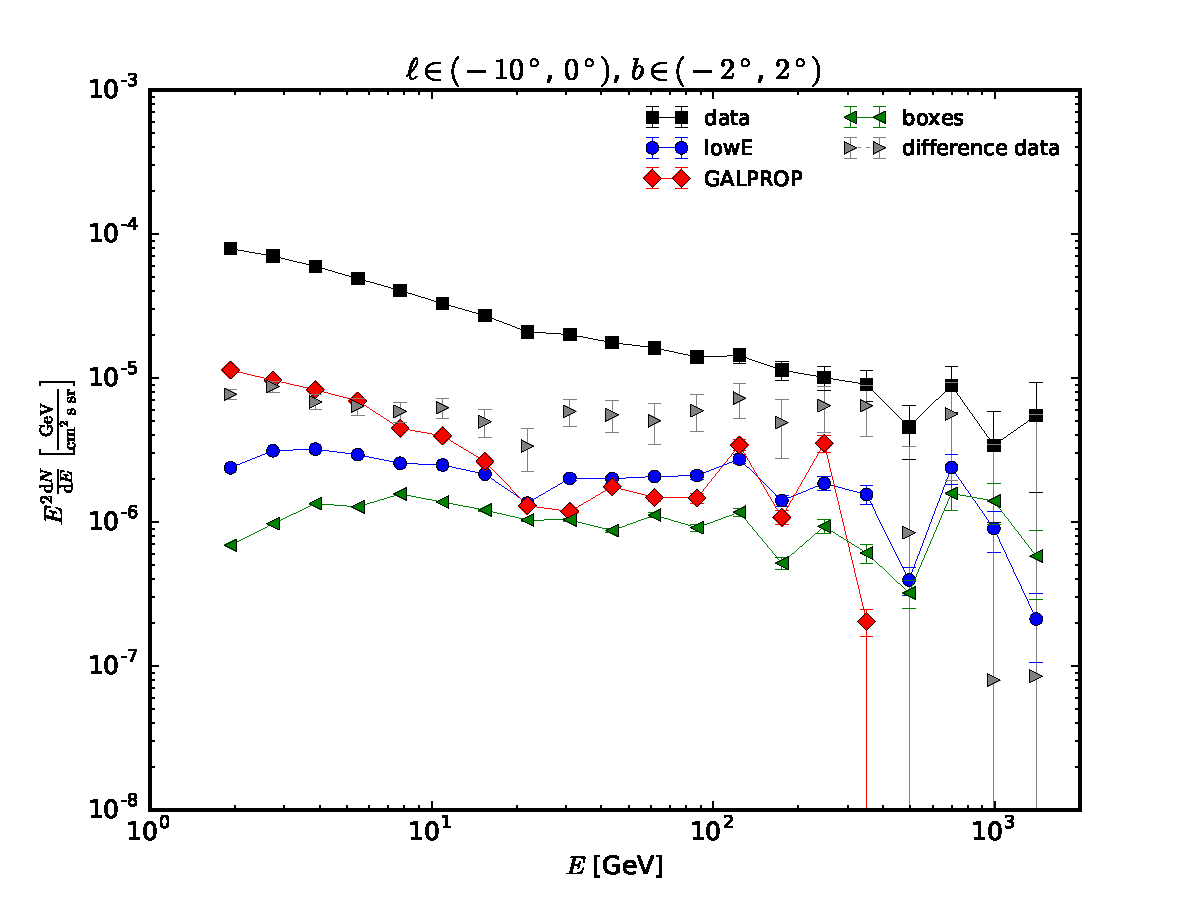
\includegraphics[width=.95\textwidth]{plots/SED_all_left-right__l=-5_b=0.pdf}
%	\end{subfigure}%
%}
%\vspace*{-0.2cm}
%	\makebox[\linewidth][c]{%
%		\begin{subfigure}[b]{.4\textwidth}
%		\centering 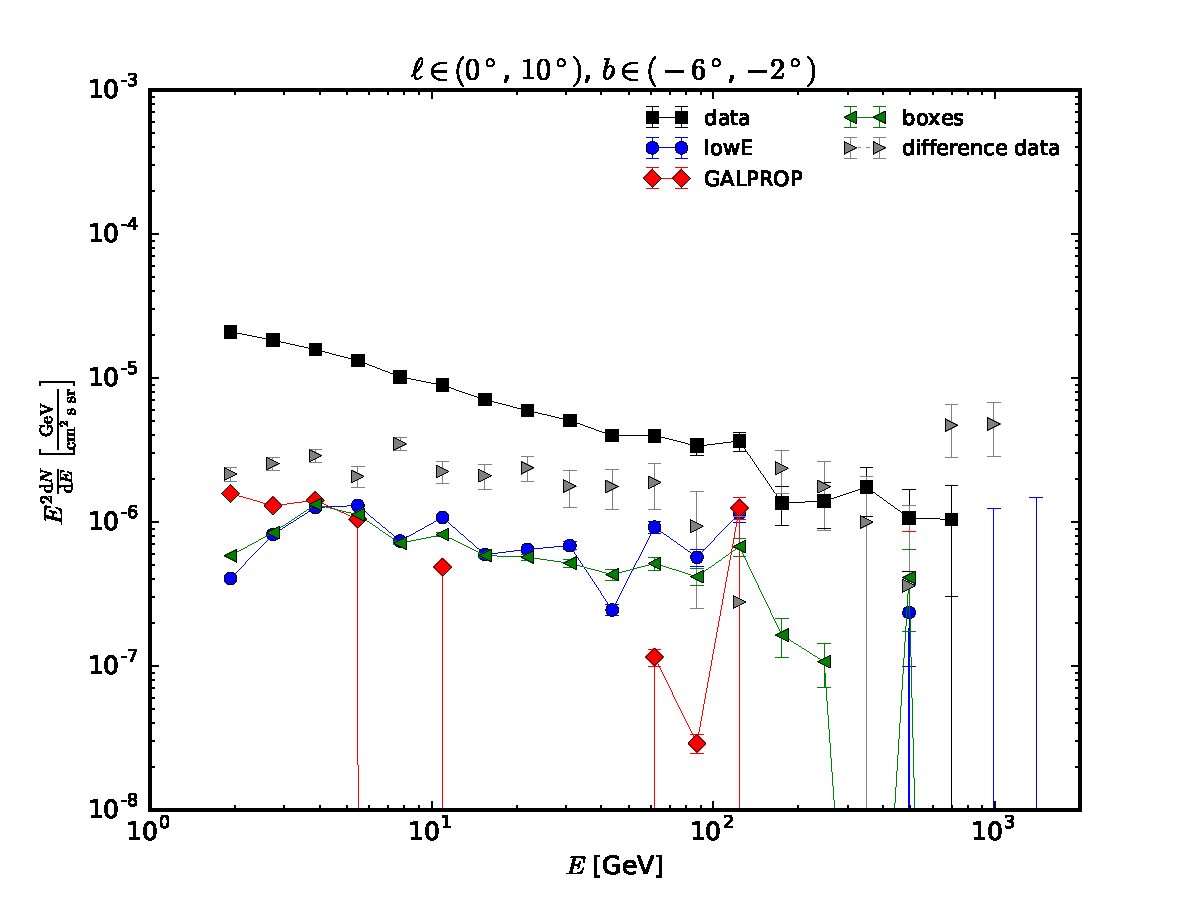
\includegraphics[width=.95\textwidth]{plots/SED_all_left-right__l=5_b=-4.pdf}
%		\end{subfigure}%
%		\begin{subfigure}[b]{.4\textwidth}
%		\centering 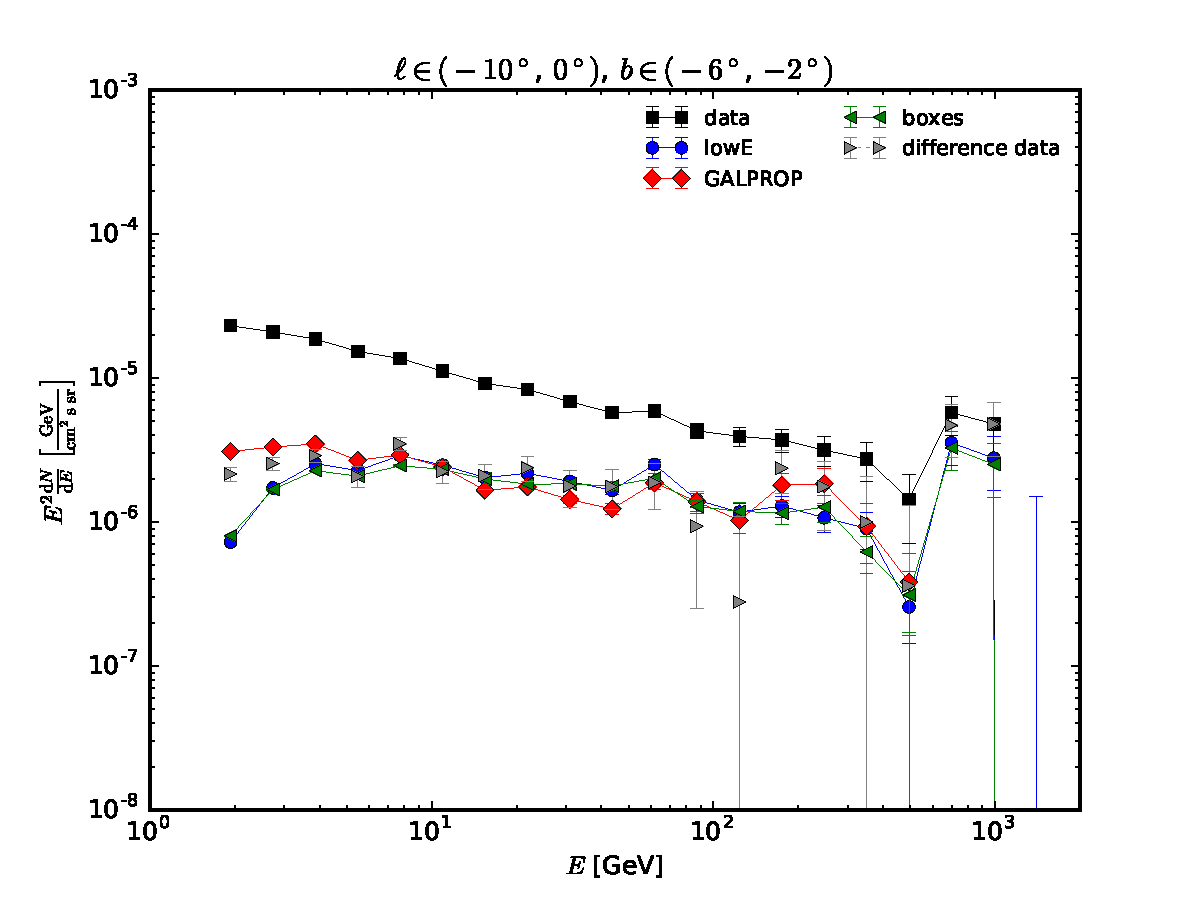
\includegraphics[width=.95\textwidth]{plots/SED_all_left-right__l=-5_b=-4.pdf}
%	\end{subfigure}%
%}
%\vspace*{-0.2cm}
%	\makebox[\linewidth][c]{%
%		\begin{subfigure}[b]{.4\textwidth}
%		\centering 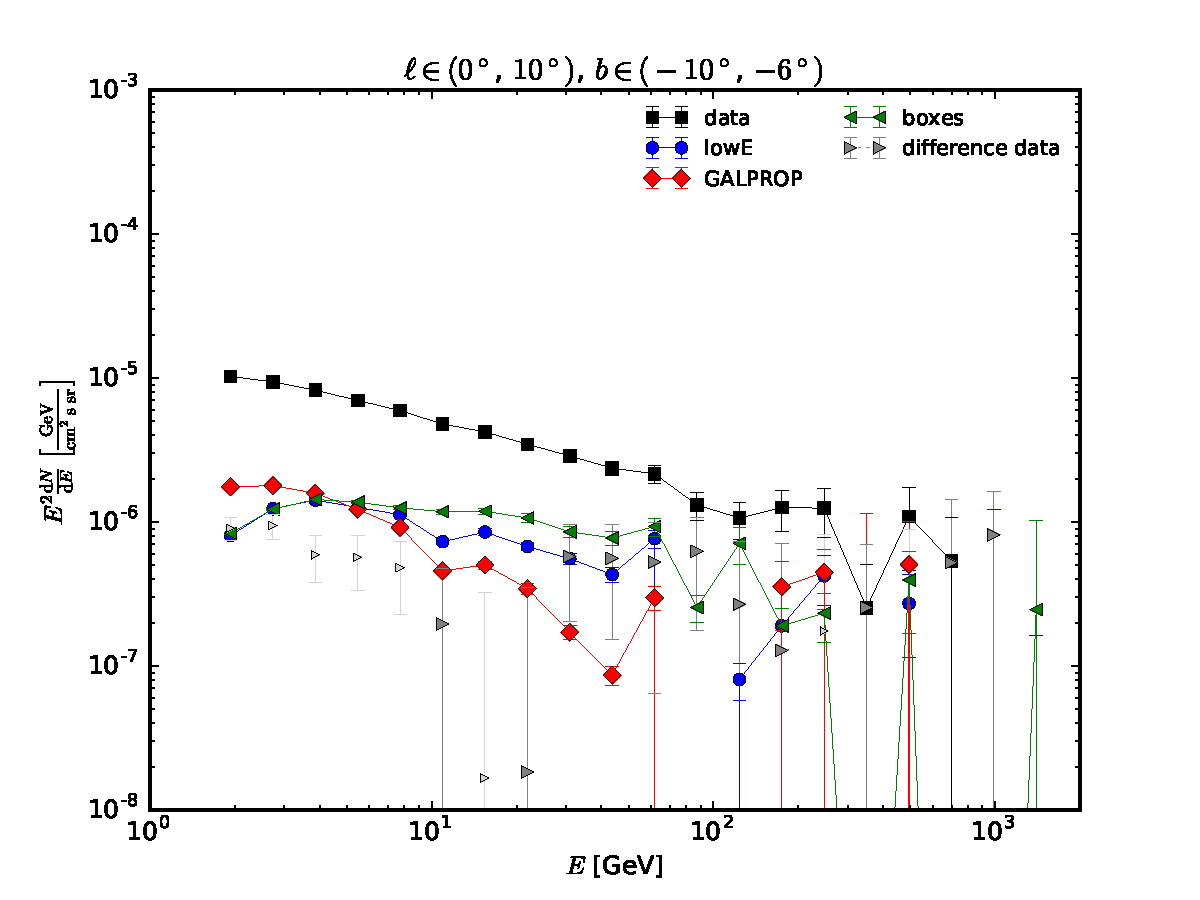
\includegraphics[width=.95\textwidth]{plots/SED_all_left-right__l=5_b=-8.pdf}
%		\end{subfigure}%
%		\begin{subfigure}[b]{.4\textwidth}
%		\centering 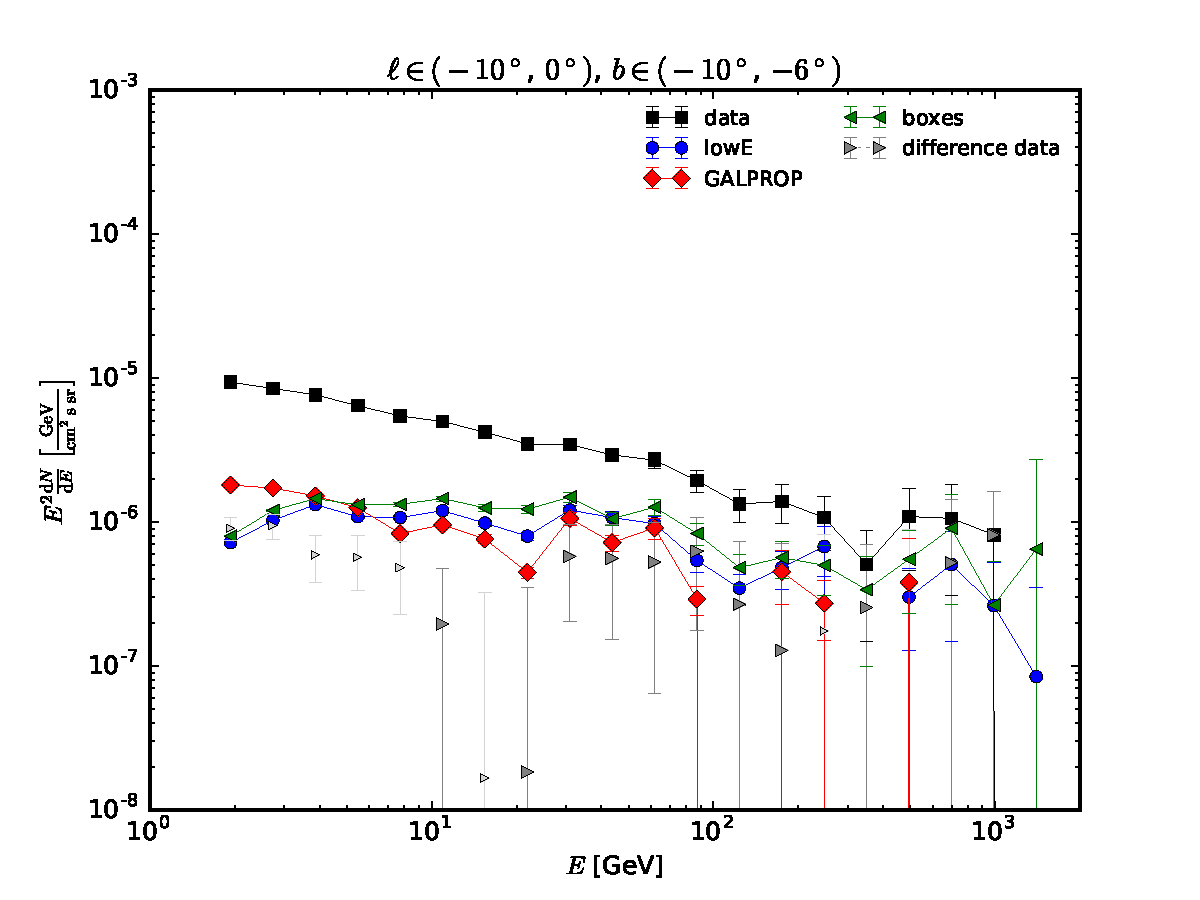
\includegraphics[width=.95\textwidth]{plots/SED_all_left-right__l=-5_b=-8.pdf}
%	\end{subfigure}%
%}
%\caption{Spectra.}
%\label{Spectra_all}
%\end{figure*}



\subsection{IC model}

Discuss the IC model.


\subsection{Pion model}